% =====================================================================
%  Основное содержимое отчёта.
% =====================================================================

\labpart{Структура разработанной системы}

Определение языка текста реализовано как новый сценарий использования
поверх уже существующей архитектуры ЛР1 (см. \texttt{docs/ARCHITECTURE.md}):
границы сервисов по-прежнему проведены по зоне ответственности, а не по
лабораторной работе, поэтому ЛР2 добавляет один новый сервис и новые
таблицы БД, не создавая отдельной инфраструктуры. Структура системы на
уровне контейнеров (C4, уровень 2) показана на
рисунке~\ref{fig:architecture-c4}; компоненты и связи, добавленные
именно в этой лабораторной работе, выделены зелёным цветом и вынесены
отдельным пунктом легенды.

\pumldiagram{architecture-c4}{Диаграмма контейнеров разработанной системы (нотация C4); зелёным -- новое в ЛР2}{architecture-c4}{0.95}

Новый сервис \texttt{lang-id-service} (Python, FastAPI + PyTorch) --
углублённый элемент варианта 25 (реализация методов распознавания
языка). Он не хранит состояние и не обращается к БД самостоятельно: как
и \texttt{nlp-service}, он получает на вход уже подготовленные данные
(тексты для построения профиля, координаты весов классификатора) и
возвращает чистый результат вычисления -- профиль языка или решение о
языке одного текста. Оркестрацией (какие профили есть, какие документы
размечены, что показывать пользователю) занимается \texttt{api}, как и
для остальных сценариев системы. Помимо нового сервиса, ЛР2 расширила
ответственность трёх уже существующих компонентов:
\begin{itemize}
  \item \textbf{frontend} получил новую страницу «Язык» с четырьмя
  вкладками (разметка, профили, ручная проверка, тестирование);
  \item \textbf{crawler-service} и модель \texttt{CrawlSeed} стали
  поддерживать язык обхода не на уровне коллекции, а на уровне каждого
  стартового адреса (\texttt{CrawlSeed.language}) -- это позволяет
  наполнять одну коллекцию сразу несколькими языковыми Wikipedia
  одновременно, автоматически проставляя каждому документу язык его
  источника;
  \item в \texttt{packages/nlp\_core} (переиспользуемая библиотека,
  общая для \texttt{nlp-service}, \texttt{crawler-service} и
  \texttt{api}) добавлены чистые функции построения профилей для
  лексических методов (\texttt{frequent\_words.py}, \texttt{alphabetic.py})
  и извлечение основного содержимого HTML-страницы
  (\texttt{content\_extraction.py}) -- общее и для массового краулинга, и
  для разовой проверки произвольного URL.
\end{itemize}

\labpartbreak{Структура базы данных}

Схема ключевых таблиц и связей между ними показана на
рисунке~\ref{fig:database-erd} (нотация Crow's Foot); таблицы, добавленные
в ЛР2, выделены зелёным.

\pumldiagram{database-erd}{ER-диаграмма базы данных (нотация Crow's Foot); зелёным -- новое в ЛР2}{database-erd}{1.0}

Структуры данных для входной и выходной информации метода определения
языка:
\begin{itemize}
  \item \textbf{вход (обучающая коллекция)} -- поле
  \texttt{documents.confirmed\_language} хранит человеком подтверждённый
  истинный язык документа (это и есть эталонная разметка ЛР2, аналог
  \texttt{relevance\_judgments} из ЛР1), а \texttt{documents.corpus\_split}
  ($\in \{\texttt{train}, \texttt{test}, \texttt{NULL}\}$) относит
  размеченный документ к обучающей или тестовой выборке;
  \item \textbf{вход (обученная модель)} -- таблица
  \texttt{lang\_id\_profiles}: одна строка на пару (метод, язык) для
  лексических методов, и одна строка с \texttt{language = NULL} для
  нейросетевого метода (у него один общий классификатор на все языки).
  Поле \texttt{profile\_data} (JSON) хранит то, что нужно конкретному
  методу -- ранжированный список слов, распределение частот букв, либо
  веса/смещения/порядок классов и кривую обучения нейросети;
  \texttt{lang\_id\_training\_jobs} хранит текущий прогресс обучения
  нейросетевого классификатора (эпоха, значение функции потерь,
  точность на обучающей выборке) для живого прогресс-бара в интерфейсе;
  \item \textbf{выход (результат одного прогона тестирования)} --
  \texttt{lang\_id\_runs} (одно тестирование одного метода на тестовой
  выборке коллекции) и \texttt{lang\_id\_results} (результат по каждому
  документу: предсказанный язык, расстояния до профиля каждого языка,
  затраченное время, совпадение с \texttt{confirmed\_language});
  \item \textbf{выход (агрегат)} -- \texttt{lang\_id\_run\_metrics}
  хранит посчитанные по прогону Accuracy/Precision/Recall/F1, по
  аналогии с тем, как \texttt{metric\_results} кеширует метрики поиска
  в ЛР1.
\end{itemize}

\labpart{Основные алгоритмы}

Все три реализованных метода подчиняются одинаковой трёхшаговой схеме
задания: построить поисковый образ языка (ПОЯ) по обучающему корпусу,
построить поисковый образ документа (ПОД) по тем же правилам и выбрать
язык с минимальным расстоянием между ПОЯ и ПОД. Общий алгоритм показан
на рисунке~\ref{fig:lang-id-pipeline}; методы отличаются только
правилом построения ПОЯ/ПОД (шаг 2) и метрикой расстояния -- итоговое
правило выбора (шаг 3) для всех методов одно и то же.

\pumldiagram{lang-id-pipeline}{Алгоритм определения языка одного текста (общая схема для всех трёх методов)}{lang-id-pipeline}{0.85}

\textbf{Метод частотных слов.} ПОЯ -- список из 300 самых частых слов
обучающего корпуса языка (аналог 300 самых частых N-грамм из метода
Кавнара--Тренкла (1994), но применённый к целым словам, а не к
N-граммам символов, как того требует вариант задания). Расстояние до
ПОД документа -- сумма модулей разности рангов слова в ПОЯ и в
частотном списке слов документа (\emph{out-of-place measure}):
\begin{equation}
  d_{\text{words}}(\text{ПОЯ}, \text{ПОД}) = \sum_{w \in \text{ПОЯ}} \left|\, \mathrm{rank}_{\text{ПОЯ}}(w) - \mathrm{rank}_{\text{ПОД}}(w) \,\right|,
\end{equation}
где слову ПОЯ, отсутствующему в документе, назначается штраф, равный
размеру самого ПОЯ (300) -- он заведомо больше любого реального
рассогласования рангов внутри списка.

\textbf{Алфавитный метод.} ПОЯ -- нормированное распределение частот
букв обучающего корпуса языка: $p_i = \mathrm{count}(c_i) / \sum_j \mathrm{count}(c_j)$
по всем алфавитным символам текста (\texttt{str.isalpha()}), без
привязки к фиксированному 26-буквенному латинскому алфавиту -- это
существенно для французского языка, где буквы с диакритикой (é, è, ç,
à, ...) несут различительную информацию и не сворачиваются в свой
безакцентный вариант. Расстояние -- манхэттенское (L1) между
распределениями ПОЯ и ПОД:
\begin{equation}
  d_{\text{alpha}}(\text{ПОЯ}, \text{ПОД}) = \sum_{c} \left|\, p^{\text{ПОЯ}}_c - p^{\text{ПОД}}_c \,\right|.
\end{equation}

\textbf{Нейросетевой метод.} ПОЯ и ПОД в этом методе не строятся явно
как профили языка -- вместо этого один общий классификатор
$\mathrm{softmax}(W \cdot x + b)$ (линейный слой без скрытых слоёв,
$x$ -- эмбеддинг документа Qwen3-Embedding-8B той же модели, что и
дополнительная модель поиска ЛР1) обучается сразу на всех
классифицируемых языках. Линейная архитектура (\autoref{fig:mlp_architecture}) выбрана осознанно: на
нескольких сотнях документов на язык дополнительный скрытый слой не
имеет статистической опоры и переобучится, тогда как линейный слой с
$L_2$-регуляризацией (\texttt{weight\_decay} в оптимизаторе Adam)
математически эквивалентен мультиномиальной логистической регрессии --
разумная модель для данного объёма данных при полноценном цикле
обучения (200 эпох, разбитых на чанки по 10 для живого прогресс-бара).
«Расстоянием» до языка $l$ для единообразия с двумя другими методами
считается $d_{\text{neural}}(l) = 1 - P(l \mid x)$, так что правило
«язык с минимальным расстоянием» остаётся общим для всех методов
(\texttt{app.domain.lang\_id}).


\begin{figure}[H]
  \centering
  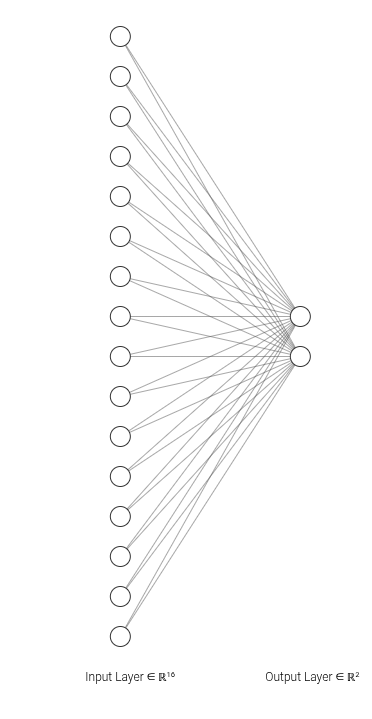
\includegraphics[width=0.2\textwidth]{lab/pictures/mlp_model.png}
  \caption{Архитектура нейронной сети для классификации языка (4096 нейронов на входном слое, 2 на выходном)}
  \label{fig:mlp_architecture}
\end{figure}

\textbf{Оценка качества.} Для каждого метода и каждого документа
тестовой выборки известны истинный язык (\texttt{confirmed\_language})
и предсказанный. Из пар (истинный, предсказанный) строится матрица
ошибок, по которой считаются точность (Accuracy, доля верных
предсказаний), Precision/Recall/F1 отдельно для каждого языка, а затем
их среднее по всем языкам (макро-усреднение) -- рекомендованный подход,
когда языки представлены в тестовой выборке неравными долями.

\labpartbreak{Тестовая коллекция документов}

Согласно методическим указаниям, тестовая коллекция сформирована на
основании многоязычных статей Wikipedia. Коллекция \texttt{Wikipedia}
наполнена двумя независимыми запусками обхода, каждый ограничен своим
доменом: с \texttt{en.wikipedia.org} (глубина 3, лимит 500 документов,
переход только в пределах домена) и с \texttt{fr.wikipedia.org}
(глубина 3, лимит 500 документов, переход только в пределах домена) --
итого 1000 документов, каждый автоматически помечен языком своего
seed'а. Каждому документу вручную подтверждён истинный язык (истинный
язык у всех документов совпал с языком seed'а, из которого он получен,
что ожидаемо для обхода внутри одного языкового раздела Wikipedia) и он
отнесён к обучающей или тестовой выборке -- кнопкой автоматического
стратифицированного разбиения (80\,\%/20\,\% отдельно по каждому
языку, чтобы оба языка были представлены в обеих выборках
пропорционально) либо вручную по каждому документу
(\autoref{fig:language-labeling}): итого 800 документов в обучающей
выборке (400 на английском, 400 на французском) и 200 в тестовой (по
100 на язык).

\begin{figure}[H]
  \centering
  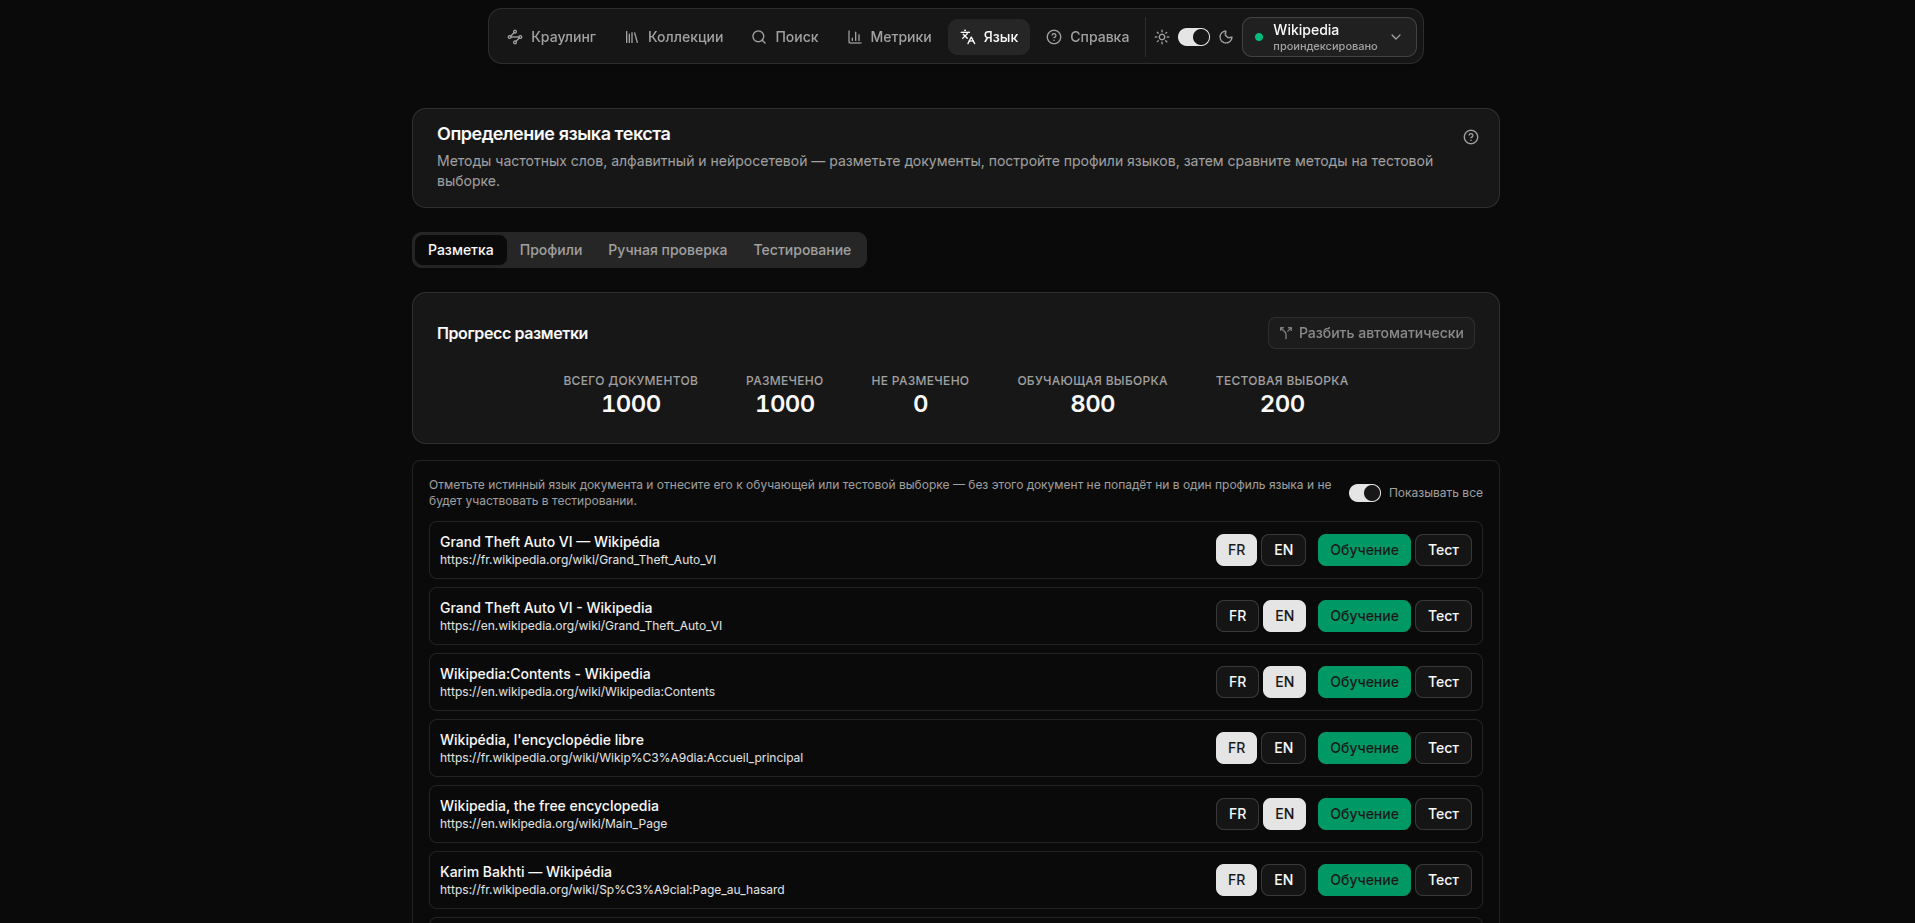
\includegraphics[width=0.85\textwidth]{lab/pictures/language_labeling.png}
  \caption{Вкладка «Разметка»: прогресс разметки коллекции и назначение истинного языка/выборки каждому документу}
  \label{fig:language-labeling}
\end{figure}

По обучающей выборке построены профили обоих лексических методов для
каждого языка (\autoref{fig:language-profiling}) и обучен единый
нейросетевой классификатор на всех 800 обучающих документах сразу.

\begin{figure}[H]
  \centering
  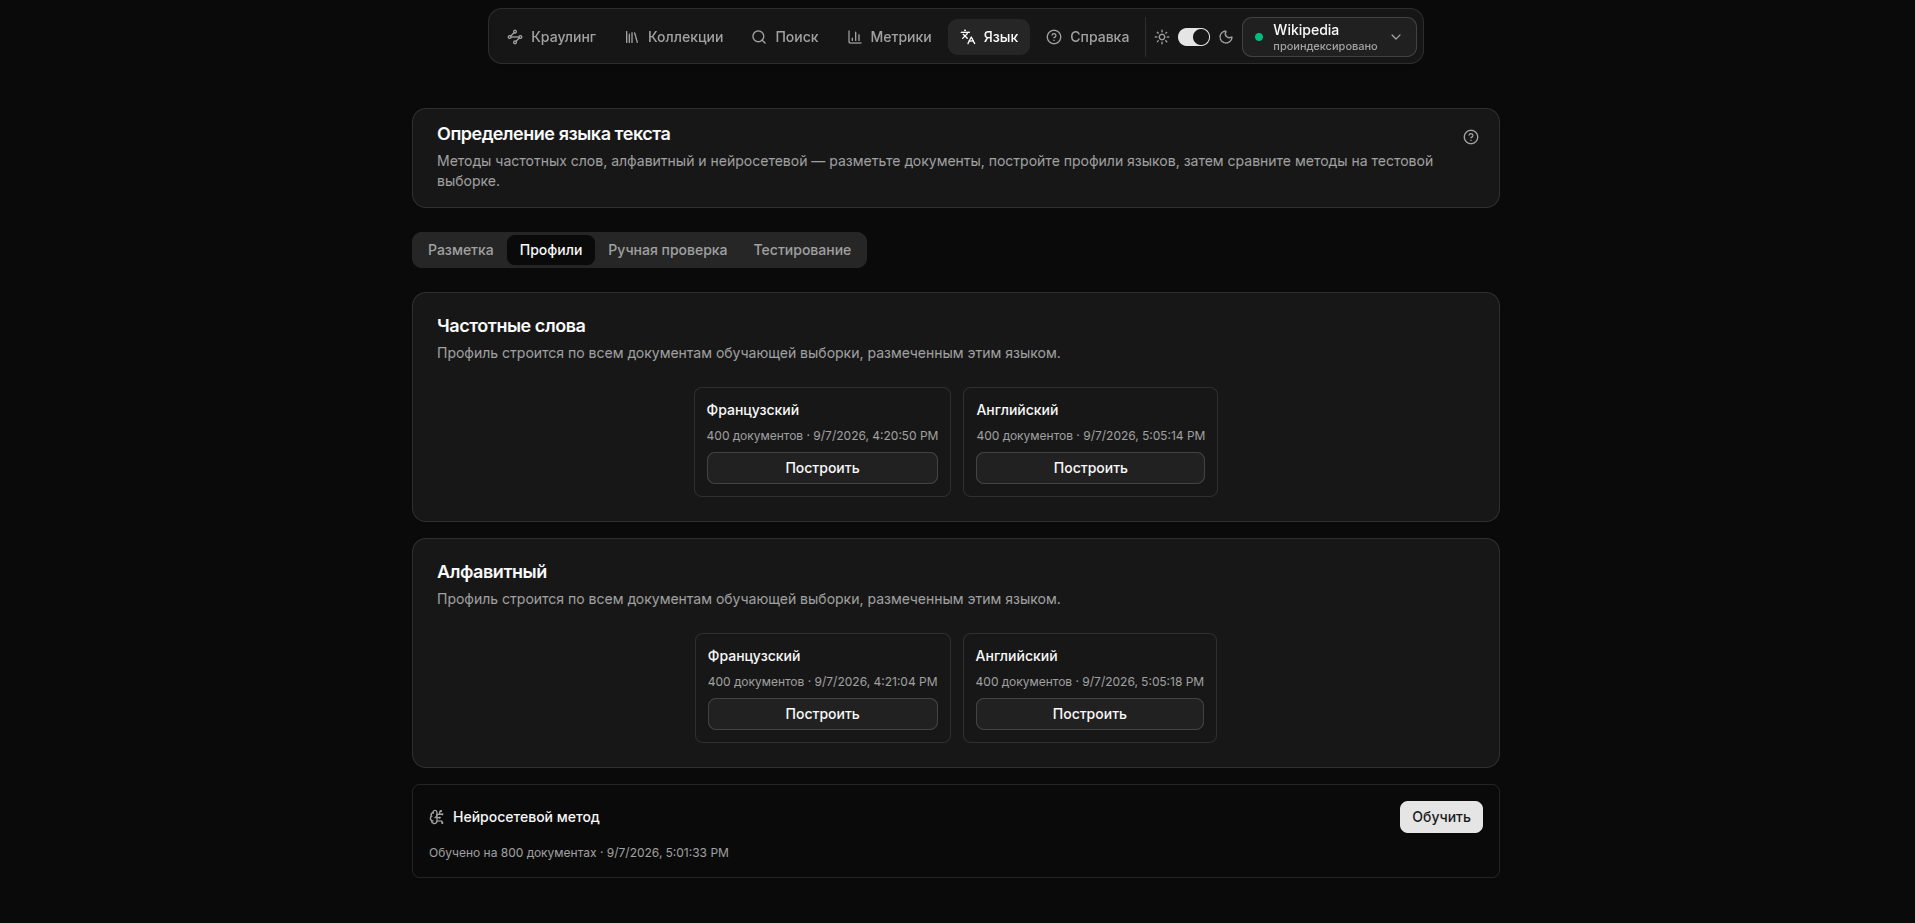
\includegraphics[width=0.85\textwidth]{lab/pictures/language_profiling.png}
  \caption{Вкладка «Профили»: построенные профили частотных слов и алфавитные профили по каждому языку, обученный нейросетевой классификатор}
  \label{fig:language-profiling}
\end{figure}

\labpart{Результаты тестирования и оценка качества}

Каждый из трёх методов протестирован на одной и той же тестовой
выборке из 200 документов (100 английских, 100 французских), не
пересекающейся с обучающей. Средние по документам метрики приведены в
таблице~\ref{tab:metrics-langid}; тот же расчёт в интерфейсе системы --
на рисунках~\ref{fig:methods-comparison} (вкладка «Тестирование») и
\ref{fig:language-metrics} (страница «Метрики»).

\begin{table}[H]
  \centering
  \caption{Метрики качества и быстродействия по 200 документам тестовой выборки}
  \label{tab:metrics-langid}
  \begin{tabularx}{\textwidth}{|X|r|r|r|}
    \hline
    Метрика & Частотные слова & Алфавитный & Нейросетевой \\
    \hline
    Accuracy & 95{,}5\,\% & 100{,}0\,\% & 100{,}0\,\% \\
    \hline
    Precision (macro) & 95{,}7\,\% & 100{,}0\,\% & 100{,}0\,\% \\
    \hline
    Recall (macro) & 95{,}5\,\% & 100{,}0\,\% & 100{,}0\,\% \\
    \hline
    F1 (macro) & 95{,}5\,\% & 100{,}0\,\% & 100{,}0\,\% \\
    \hline
    Среднее время классификации & 3{,}96 мс & 4{,}97 мс & 1{,}24 мс \\
    \hline
  \end{tabularx}
\end{table}

\begin{figure}[H]
  \centering
  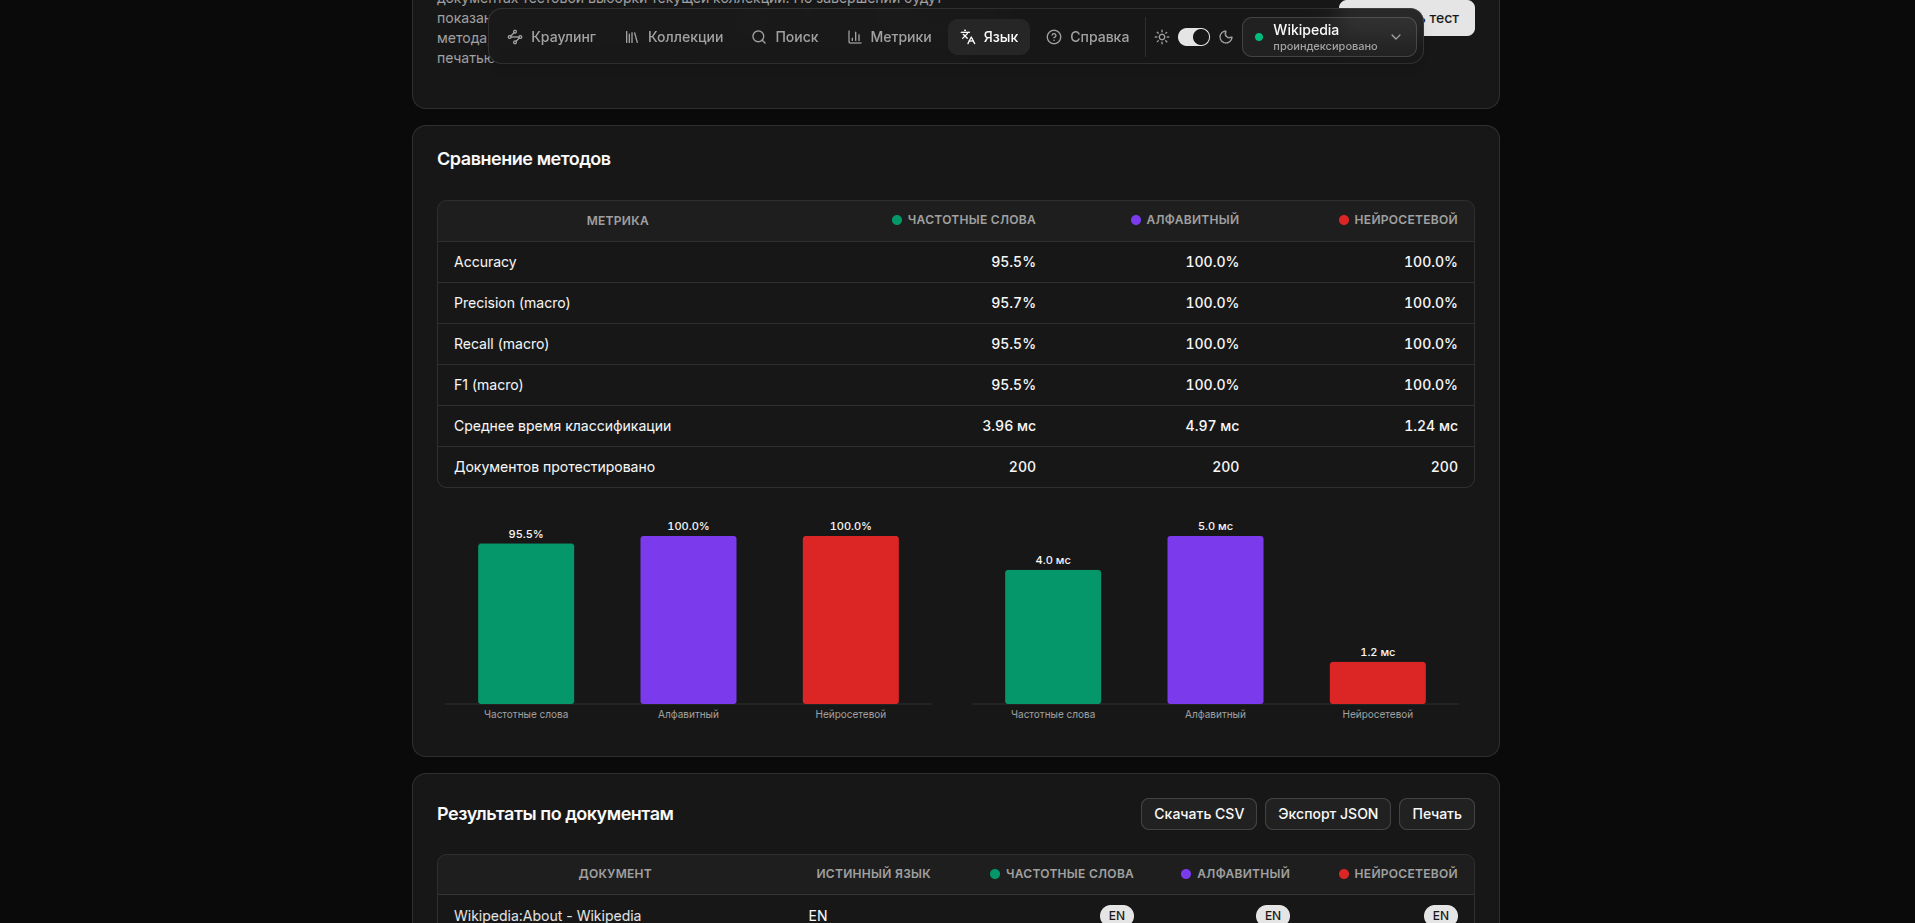
\includegraphics[width=\textwidth]{lab/pictures/methods_comparison.png}
  \caption{Вкладка «Тестирование»: сравнение методов по точности и времени, результаты по документам с экспортом (CSV/JSON) и печатью}
  \label{fig:methods-comparison}
\end{figure}

\begin{figure}[H]
  \centering
  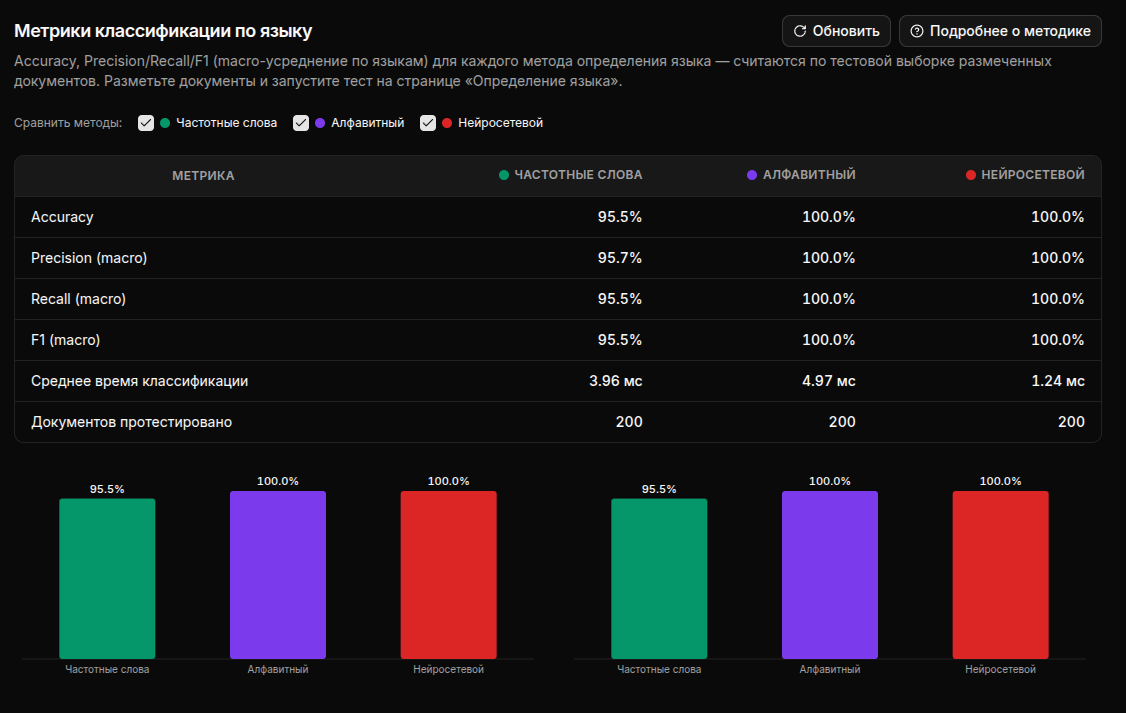
\includegraphics[width=0.85\textwidth]{lab/pictures/language_metrics.png}
  \caption{Раздел «Метрики классификации по языку» на странице «Метрики» -- тот же расчёт, что и на вкладке «Тестирование», с возможностью пересчёта}
  \label{fig:language-metrics}
\end{figure}

Отдельно от прогона по тестовой выборке система поддерживает разовую
проверку одного текста -- по адресу веб-страницы (основное содержимое
которой извлекается тем же алгоритмом Readability, что и при массовом
краулинге, без создания документа в коллекции) или по вставленному/
загруженному тексту, сразу всеми тремя методами
(\autoref{fig:hand-check}). Результат разовой проверки, как и результат
тестового прогона, можно выгрузить в CSV/JSON или распечатать.

\begin{figure}[H]
  \centering
  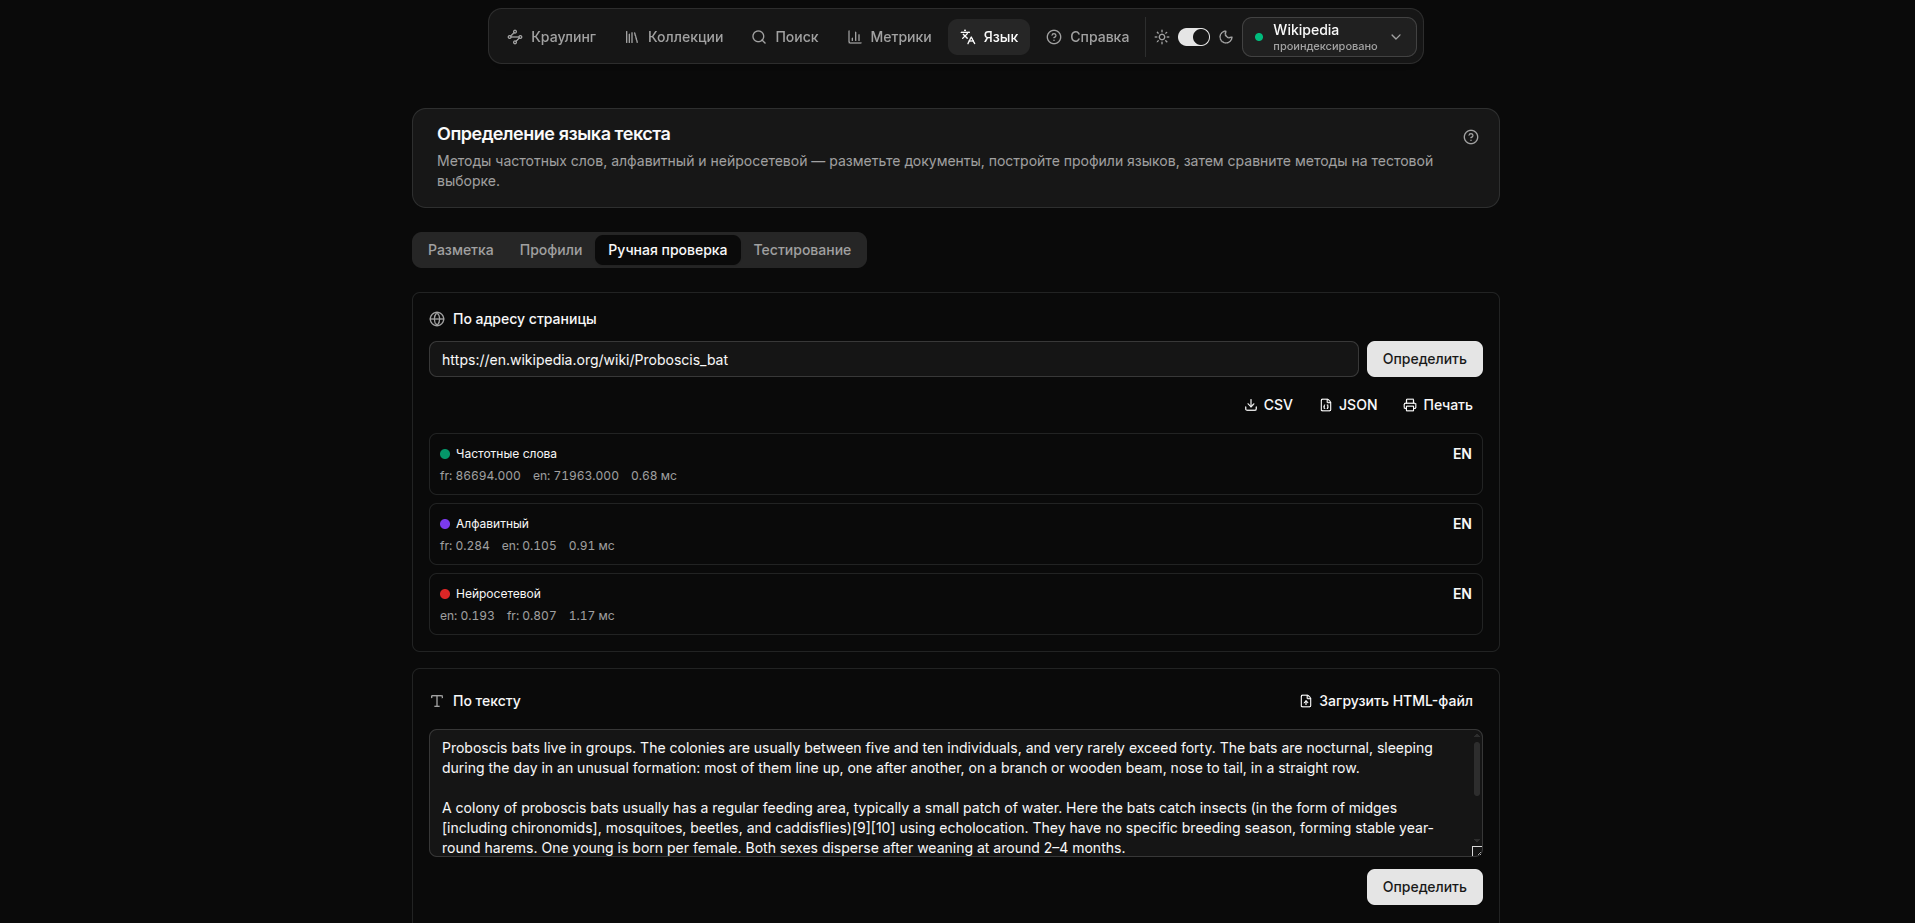
\includegraphics[width=0.85\textwidth]{lab/pictures/hand_check.png}
  \caption{Вкладка «Ручная проверка»: определение языка по адресу страницы всеми тремя методами с расстояниями и временем}
  \label{fig:hand-check}
\end{figure}

\labpart{Анализ результатов и предложения по улучшению}

\begin{enumerate}
  \item \textbf{Оба языковых профиля разошлись у метода частотных
  слов реже, чем у остальных двух.} На паре английский/французский
  алфавитный и нейросетевой методы дали 100\,\% точность на всех 200
  тестовых документах -- ожидаемый результат: у английского и
  французского языков заметно разное распределение частот букв
  (диакритические знаки, иные пропорции гласных) и разделимые в
  векторном пространстве эмбеддинги, поэтому оба сигнала оказались
  практически линейно разделимыми на этой паре языков. Метод частотных
  слов ошибся на $\approx$4,5\,\% документов -- вероятная причина:
  фрагменты статей Wikipedia, где часто встречаются вставки на другом
  языке (имена собственные, цитаты, интервики-ссылки), сдвигающие
  ранги слов сильнее, чем распределение букв или семантику текста в
  целом.
  \item \textbf{Нейросетевой метод при этом быстрее обоих лексических.}
  Среднее время классификации одного документа -- 1{,}24~мс у
  нейросетевого метода против 3{,}96~мс (частотные слова) и 4{,}97~мс
  (алфавитный, \autoref{tab:metrics-langid}). Причина -- у нейросетевого
  метода на этапе классификации выполняется единственный прямой проход
  через линейный слой над уже готовым эмбеддингом, тогда как лексические
  методы заново токенизируют/анализируют посимвольно весь текст
  документа при каждой проверке.
  \item \textbf{Что можно добавить в систему для её улучшения.}
  \begin{itemize}
    \item расширение количества классифицируемых языков (сейчас два) --
    архитектура методов (профиль на язык у лексических методов, число
    выходных классов у нейросетевого) уже рассчитана на произвольное
    число языков, ограничение только в количестве размеченных данных;
    \item метод N-грамм символов (в дополнение к уже реализованному
    методу частотных слов) -- по вариантам задания это тот же класс
    методов, что и частотные слова, но устойчивее к языкам с богатой
    морфологией, где словоформа реже повторяется буквально;
    \item доверительный порог (confidence threshold) для нейросетевого
    метода -- отдельный класс «не удаётся определить» для документов, у
    которых вероятность лучшего языка низкая, вместо всегда
    принудительного выбора одного из известных языков;
    \item кросс-валидация по нескольким случайным стратифицированным
    разбиениям вместо одного фиксированного train/test -- сейчас 100\,\%
    точность алфавитного и нейросетевого методов может быть отчасти
    объяснена удачным разбиением, а не только качеством методов.
  \end{itemize}
  \item \textbf{Где систему можно применить.}
  \begin{itemize}
    \item предварительная фильтрация языка документов перед их
    попаданием в коллекцию поиска ЛР1 -- например, автоматическая
    маршрутизация англо- и франкоязычных страниц в раздельные индексы
    вместо смешанного мультиязычного индекса;
    \item модерация многоязычных пользовательских данных (комментарии,
    обращения в поддержку) -- быстрая маршрутизация по языку без
    привлечения тяжёлых моделей перевода;
    \item учебный полигон для последующих лабораторных работ курса,
    использующих понятие языка документа (машинный перевод, синтез и
    распознавание речи) -- размеченный по языку корпус и профили уже
    хранятся в общей БД и переиспользуемы.
  \end{itemize}
\end{enumerate}

\labpartbreak{Использованные готовые компоненты}

\begin{table}[H]
  \centering
  \caption{Библиотеки и программные средства, использованные при реализации ЛР2 (дополнительно к перечисленным в отчёте по ЛР1)}
  \label{tab:stack-langid}
  \small
  \begin{tabularx}{\textwidth}{|l|X|}
    \hline
    Компонент & Назначение \\
    \hline
    PyTorch (\texttt{torch.nn.Linear} + \texttt{softmax}) & Нейросетевой
      классификатор языка: обучение (Adam, $L_2$-регуляризация) и
      инференс поверх готовых эмбеддингов документа. \\
    \hline
    readability-lxml & Извлечение основного содержимого HTML-страницы
      (алгоритм Mozilla Readability, тот же, что в Firefox Reader View)
      перед определением языка произвольного URL и перед очисткой
      страниц при краулинге -- убирает навигацию, подвал и рекламные
      блоки, оставляя только текст статьи. \\
    \hline
    Qwen3-Embedding-8B (через OpenRouter) & Источник плотных векторных
      представлений документа для нейросетевого метода -- та же модель,
      что и в дополнительной модели поиска ЛР1; эмбеддинги, посчитанные
      при индексации коллекции для поиска, переиспользуются без
      повторного обращения к OpenRouter. \\
    \hline
  \end{tabularx}
\end{table}
